\documentclass[a4paper, 10pt, twocolumn]{jarticle}
\pagestyle{empty}

\usepackage[dvipdfmx]{graphicx}
\usepackage[top=20truemm, bottom=20truemm, left=18truemm, right=18truemm]{geometry}
\usepackage{calc}
\usepackage{titlesec}
\usepackage{amsmath}

\setlength{\columnsep}{\columnsep + 4zw}
\setlength{\textheight}{49\baselineskip}
\titleformat*{\section}{\normalsize\bfseries}
\titleformat*{\subsection}{\normalsize\bfseries}

\titlespacing{\section}{0pt}{4pt}{4pt}
\titlespacing{\subsection}{0pt}{4pt}{4pt}
\setlength{\intextsep}{10pt}
\setlength{\textfloatsep}{10pt}

\linespread{0.90} % 行間を0.9倍に設定


\begin{document}
\twocolumn
[
    \centering
    \vspace{0.5\baselineskip}
    {\large\bfseries
        様々な環境や状況に\\対応できるPDRベースの\\3次元屋内位置推定\\ライブラリに関する研究
    } \\
    \vspace{0.5\baselineskip}
    B23714 外山瑠起 指導教員 梶克彦 \\
    \vspace{\baselineskip}
    キーワード: 屋内位置推定,PDR,ライブラリ
    \vspace{\baselineskip}
    \vspace{\baselineskip}
]


\section{はじめに}


屋内環境における位置推定は,様々なサービスや業務の基盤として重要性を増している.
大規模商業施設での顧客誘導,物流倉庫での作業効率化など,その応用範囲は広がり続けている.
しかし,屋内ではGPSなどの衛星測位システムの利用が難しく,代替となる位置推定手法が必要とされる.

% TODO: IMUの所の文章少し違和感
屋内位置推定手法は主に,絶対位置推定と相対位置推定に大別される.
絶対位置推定は空間内での絶対的な位置を求める手法であり,
Wi-FiやBLEビーコンなどの電波を用いた手法がある.
相対位置推定は特定の基準点からの相対的な位置を求める手法であり,
代表的な手法であるPDR(Pedestrian Dead Reckoning)は,
IMU(慣性計測装置)から得られる加速度と角速度を用いて歩行者の移動を推定する.
近年ではPDRと電波強度を組み合わせた手法\cite{pdr-rss-fusion}や,
フロアマップ情報を活用したマップマッチング手法\cite{pdr-map}など,
複数の手法を統合したアプローチが提案されている.
しかしこれらの手法の多くは特定の環境を想定して設計されており,
異なる環境への部分的な適用は困難である.

そこで本研究では様々な環境や状況に対応可能な,PDRベースの3次元屋内位置推定ライブラリの開発を目的とする.
図1に本研究で提案するライブラリの概要を示す.
本ライブラリはPDRを基盤技術として採用し,環境情報を活用した段階的な補正アプローチを導入する.
また拡張性と再利用性を重視したソフトウェアアーキテクチャを採用し,
新たな補正アルゴリズムの追加や既存アルゴリズムの組み合わせを容易にする.


\begin{figure}[h]
	\centering
	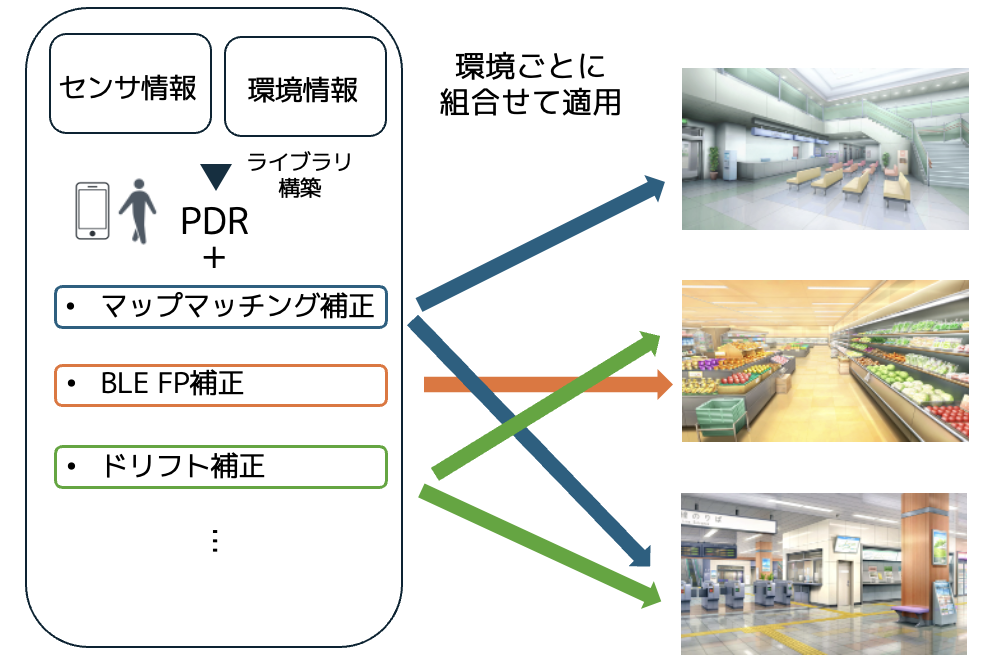
\includegraphics[width=\linewidth]{image/first.png}
	\caption{様々な環境や状況に対応できるPDRベースの\\3次元屋内位置推定ライブラリの概要}    \label{fig:overview}
\end{figure}


\section{PDRベースの3次元屋内位置推定ライブラリの検討}


\subsection{要求仕様}



屋内環境における位置推定システムの開発には,
環境条件と利用可能な補正情報の多様性を考慮する必要がある.
本ライブラリでは基本となるセンサ情報として加速度センサとジャイロセンサをPDRの基本処理に,
気圧センサを階層判定による3次元位置推定に利用する.
環境情報としては歩行可能領域の制約として機能するフロアマップ情報と,
位置推定の補正に柔軟に活用できる電波強度情報を採用する.
システムの設計においては補正アルゴリズムを独立したモジュールとして実装し,
環境に応じて適切な組み合わせが可能な設計とする.


% TODO: 背景消したいけどremove.bgすると文字の解像度が落ちる.
% 後ベクター画像になるべくしたい
\begin{figure}[h]
    \centering
    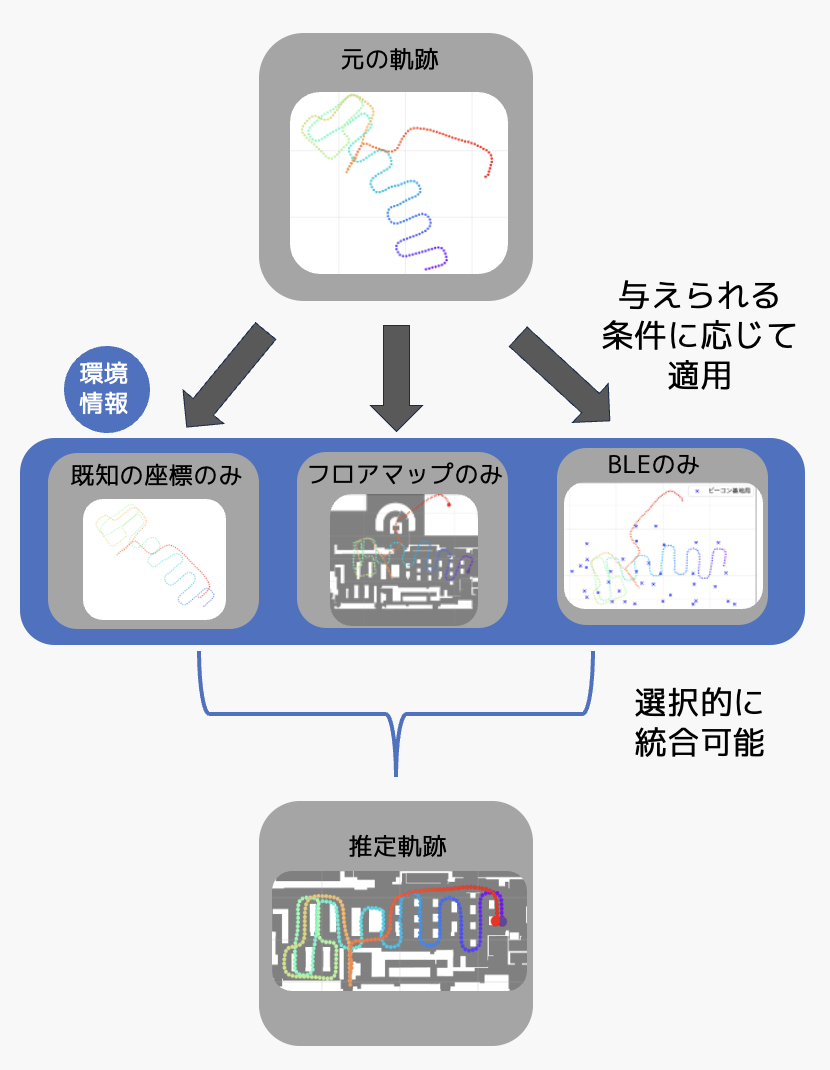
\includegraphics[width=\linewidth]{image/integrate4.jpg}
    \caption{環境条件に応じた補正の適用}
    \label{fig:corrector-class}
\end{figure}



\subsection{xDR challenge 2023における平面的な位置推定}
本ライブラリの補正アルゴリムの検討及び検証として,PDRベンチマーク標準化委員会が主催する
xDR Challenge 2023\footnote{産業技術総合研究所,https://unit.aist.go.jp/harc/xDR-Challenge-2023/(2023年10月)}の環境を用いた.
このコンテストでは,高速道路のサービスエリアを対象とし,被験者がスマートフォンとハンドヘルドLiDARを保持して歩行する.
スマートフォンからは各種センサデータとBLEビーコンの受信電波強度が,LiDARからは正解軌跡が取得される.

PDRによる初期推定では,加速度の大きさから歩行タイミングを検出し,角速度の積分により進行方向を推定する.
図2に示すように,この初期軌跡に対して環境条件に応じた補正を選択的に適用する.
既知の座標のみが利用可能な場合は,センサの累積誤差を低減するドリフト補正を適用する.
フロアマップ情報が利用可能な場合は,建物の構造的特徴を活用して初期進行方向を補正し,
さらに歩行可能領域の情報から軌跡を修正する.BLEビーコンが設置されている場合は,
電波強度情報を用いた2つのアプローチによる補正を提供する.一つは送信機の基地局位置を既知とし,受信強度の閾値処理と距離の最適化により軌跡を補正する手法であり,もう一つはフィンガープリントを用いた手法である.

これらの補正手法は環境に応じて選択的に統合も可能である.例えば,
フロアマップとBLEビーコンの両方が利用可能な環境では,まず建物の構造を考慮した補正を行い,
その後電波強度情報による補正を適用する.図2の下部に示すように,複数の環境情報を用いた
補正の適切な組み合わせによってより正確な推定軌跡が得られる.
このように本ライブラリは,利用可能な環境情報に応じて柔軟な補正を実現する.



\subsection{気圧データを用いた3次元的な位置推定}
屋内環境における3次元的な位置推定において,ユーザの階層の把握は重要な課題である.
本ライブラリではスマートフォンの気圧センサから得られるデータを活用し,
PDRによる2次元軌跡に階層情報を付加する手法を実装している.

気圧データを用いた階層検知には,センサのノイズや環境変化による課題が存在する.
これらに対処するため,本ライブラリでは安定区間検出とクラスタリングを組み合わせた2段階の手法を採用している.
まず気圧の変動が小さい安定区間を検出し,次にDBSCANアルゴリズムを適用して階層のグルーピングを行う.
また階層間の遷移は,安定区間の間に観測される顕著な気圧変化として検出される.
これにより,商業施設やオフィスビルなど,複数階層を有する建物内での継続的な位置推定を実現する.



\section{評価と他環境での検討}

\subsection{xDR Challenge 2023 環境での評価}
本ライブラリの評価として,xDR Challenge 2023の評価フレームワークを用いた検証を行った.
このフレームワークでは,円形誤差(l\_ce),局所空間における円形精度(l\_ca),誤差蓄積勾配(l\_eag),速度誤差(l\_ve),障害物回避要件(l\_obstacle)の5つの評価指標が用いられる.

格指標の評価結果では,100満点中l\_ce(88.55点),l\_eag(93.02点),l\_ve(95.55点),l\_obstacle(93.48点)において一定の精度を達成した.
特に速度誤差と障害物回避要件で高いスコアを記録し,
基本的なPDRアルゴリズムとフロアマップの補正が効果的に機能しているのが示された.
一方,局所空間における円形精度(l\_ca)は62.51点と低い結果となった.これは実装アルゴリズムが比較的シンプルな構成であり,
環境変化への対応力が限定的であるのを示唆している.

% \begin{table}[ht]
%     \caption{評価指数の概要}
%     \centering
%     \begin{tabular}{l|l|l}
%         \hline
%         指標 & 値(100点満点中) & 重み \\ \hline
%         l\_ce(CE:円形誤差) & 88.55 & 0.25 \\
%         l\_ca(CA\_l:局所空間における円形精度) & 62.51 & 0.20 \\
%         l\_eag(EAG:誤差蓄積勾配) & 93.02 & 0.25 \\
%         l\_ve(VE:速度誤差) & 95.55 & 0.15 \\
%         l\_obstacle(障害物回避要件) & 93.48 & 0.15 \\
%         l(総合評価指数) & 86.25 & \\ \hline
%     \end{tabular}
%     \label{table:evaluation_index}
% \end{table}


\subsection{他環境での評価}
本ライブラリの他環境への適用可能性として,駅構内と大学キャンパスでの検討を行った.駅構内では,改札の位置を利用したドリフト補正が有効である.改札は固定位置であり,ICカードの利用により通過時刻が正確に記録できる.また,フロアマップ情報も入手しやすく,マップマッチング補正の適用が期待できる.

大学キャンパスでは,Wi-Fiの基地局を活用した補正が有効である.キャンパス内には基本的にWi-Fi基地局が設置されており,新規機器設置のコストを抑えられる.ただし,基地局の正確な位置情報の把握は困難なため,フィンガープリント方式の補正が適している.また,研究室やサークルなど異なるコミュニティが混在する環境では,機器設置の申請コストも考慮が必要である.



\section{今後の課題}
PDRアルゴリズムの基本性能の向上は,引き続き重要な課題である.現状の実装では,歩行速度や路面状況の急激な変化に対する追従性に改善の余地がある.より高度な手法として,パーティクルフィルターの導入を検討している.これは複数の仮説を同時に追跡できるため,環境の不確実性に対してよりロバストな位置推定が期待できる.評価方法の拡充も重要であり,商業施設やオフィスビルなど,異なる特性を持つ環境での検証を進める必要がある.


\bibliographystyle{junsrt}
\bibliography{reference}

\end{document}

